\documentclass[a4paper, 12pt, final, garamond]{book}
\usepackage{cours-preambule}

\raggedbottom

\makeatletter
\renewcommand{\@chapapp}{Programme de kh\^olle -- semaine}
\makeatother

\begin{document}
\setcounter{chapter}{13}

\chapter{Du 09 au 13 janvier}

\section{Cours et exercices}
\section*{Ondes chapitre 1 -- Ondes progressives}
\begin{enumerate}[label=\Roman*]
    \item \textbf{Introduction}~: signal, perturbation, onde, propagation.
    \item \textbf{Onde progressive à une dimension}~: définition, représentation
        spatiale, célérité, représentation temporelle, retard, lien entre les
        représentations, formes mathématiques.
    \item \textbf{Onde progressive sinusoïdale}~: définition, double
        périodicité, rappel spectre électromagnétique, expression mathématique
        de l'OPS, vitesse de phase.
    \item \textbf{Milieux dispersifs}~: définition, exemples.
\end{enumerate}

\section{Cours uniquement}

\section*{Ondes chapitre 2 -- Interférences à deux ondes}
\begin{enumerate}[label=\Roman*]
    \item \textbf{Rappel déphasages}~: définition, valeurs particulières,
        lecture graphique.
    \item \textbf{Superposition d'ondes sinusoïdales de mêmes fréquences}~:
        introduction, signaux de même amplitude, signaux d'amplitudes
        différentes, bilan.
    \item \textbf{Approximation par une onde plane}~: sources ponctuelles,
        différence de marche, exercice d'application.
    \item \textbf{Interférences lumineuses}~: cohérence, intensité, formule de
        \textsc{Fresnel}, chemin optique/
    \item \textbf{Expérience des trous d'\textsc{Young}}~: introduction,
        présentation, détermination de l'interfrange.
\end{enumerate}

\section{Questions de cours possibles}
\begin{enumerate}
    \item Refaire l'exercice~:
\end{enumerate}
\begin{NCexem}[width=\linewidth, breakable]{Exercice}
    On considère ici un mascaret qui se déplace à la vitesse $c =
    \SI{18}{km.h^{-1}}$ le long d'un fleuve rectiligne, et on définit un axe
    $(Ox)$ dans la direction du sens de sa propagation.

    À l'instant $t=0$, le profil du niveau de l'eau du fleuve a l'allure
    suivante~:
    \begin{center}
        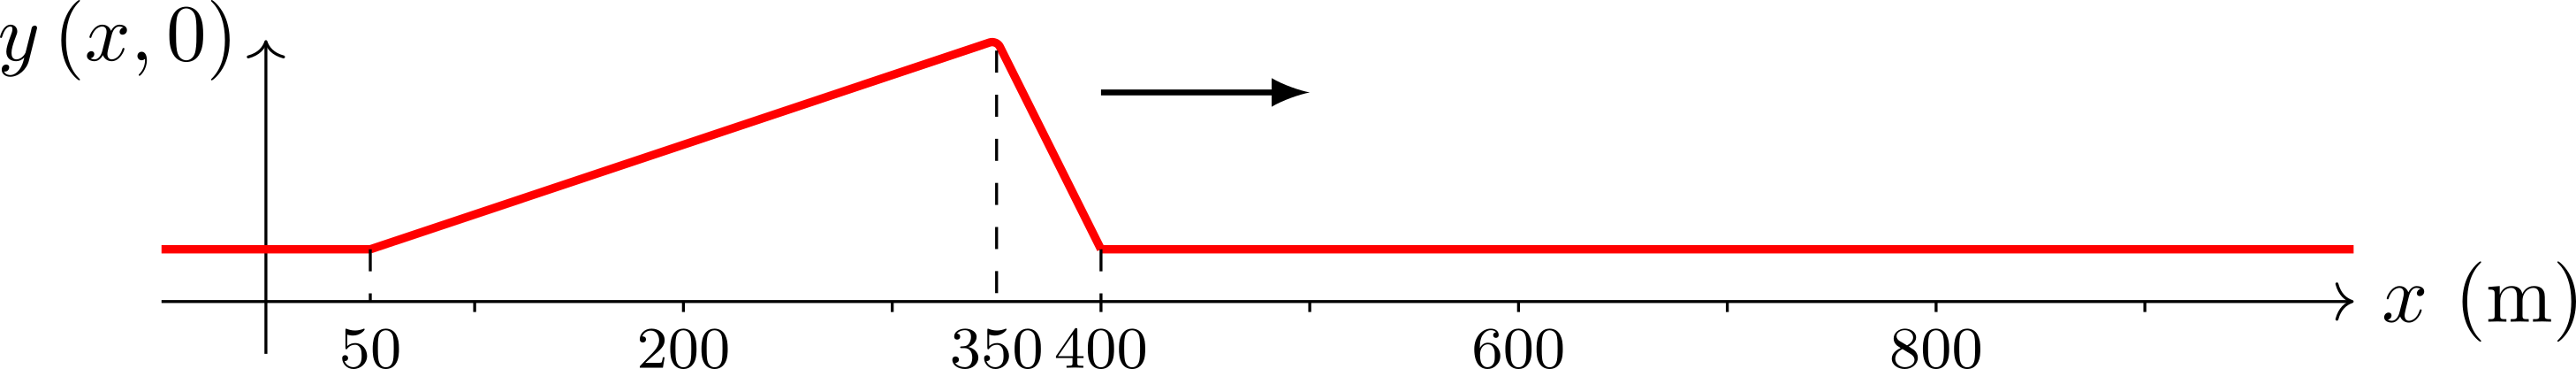
\includegraphics[width=0.8\linewidth]{rep_spa-masc_a}
    \end{center}
    \begin{enumerate}[label=\sqenumi]
        \item Faire un schéma du profil du fleuve à $\tau = \SI{1}{min}$ en
            supposant que l'onde se propage sans déformation.
        \item À quel instant la vague arrive-t-elle au point d'abscisse $x_1 =
            \SI{2.2}{km}$~? 
        \item Un détecteur fixe, enregistrant la hauteur du fleuve en fonction
            du temps, est placé à l'abscisse $x_d = \SI{1.6}{km}$. Dessiner
            l'allure des variations $y(x_d,t)$ en fonction du temps à cette
            abscisse.
    \end{enumerate}
\end{NCexem}
\begin{enumerate}[resume]
    \item Présenter ce qu'est une onde progressive sinusoïdale, établir sa
        double périodicité, indiquer les différentes relations reliant $\omega$
        et $f$ ou $T$~; $k$ et $\lambda$~; $\lambda$, $c$ et $f$ ou $T$. Définir
        un milieu dispersif et donner des exemples.
    \item Répondre à au moins 2 questions parmi les suivantes (nombre au choix
        de l'interrogataire)~:

        \begin{enumerate}
            \item Soit $f(t)$ la fonction modélisant le signal en $x=0$. Donner
                l'expression du signal en M$(x)$ ($x>0$) en considérant une onde
                qui se propage vers les $x$ croissants de O à M à la
                célérité $c$.

            \item Soit $f(t)$ la fonction modélisant le signal en $x=0$. Donner
                l'expression du signal en M$(x)$ ($x<0$) en considérant une onde
                qui se propage vers les $x$ décroissants de O à M à la
                célérité $c$.

            \item Soit $g(x)$ la fonction donnant à la date $t=0$ la valeur
                d'une grandeur physique en fonction de l'abscisse $x$ du point
                d'observation. Donner l'expression de cette grandeur en fonction
                de $x$ à la date $t$ en considérant une onde se propageant vers
                les $x$ décroissants à la célérité $c$.

            \item Une onde progressive sinusoïdale d'amplitude $A_0$ et de
                longueur d'onde $\lambda$ se propage dans le sens des $x$
                décroissants à la célérité $c$. La phase à $t=0$ au point A
                d'abscisse $x_A = {\lambda}/{4}$ est nulle. Donner l'expression
                de la fonction $s(x,t)$ en fonction de $A_0$, $\lambda$, $c$,
                $x$ et $t$. Quel est le déphasage entre A et l'origine O du
                repère~?

            \item Une onde sinusoïdale se propage dans la direction de l'axe
                $(Ox)$ dans le sens négatif avec la célérité $c$. On donne~:
                \hfill
                $\boxed{s_2(0,t) = A \sin(\omega t)}$
                \hfill~
                \smallbreak
                Déterminer l'expression de $s_2(x,t)$. Représenter graphiquement
                $s_2(\lambda/4,t)$ et $s_2(\lambda/2,t)$ en fonction de $t$.
        \end{enumerate}
    \item Refaire l'exercice~:
\end{enumerate}
\begin{NCexem}{Exercice}
    \begin{minipage}{0.55\linewidth}
        Soient 2 émetteurs sonores envoyant une onde progressive sinusoïdale de
        même fréquence, amplitude et phase à l'origine. Le premier est fixé à
        l'origine du repère, l'émetteur 2 est mobile et à une distance $d$ du
        premier, et un microphone est placé à une distance fixe $x_0$ de
        l'émetteur 1 et est aligné avec les deux émetteurs. On néglige
        l'influence de l'émetteur 2 sur l'émetteur 1 et toute atténuation.
    \end{minipage}
    \hfill
    \begin{minipage}{0.45\linewidth}
        \begin{center}
            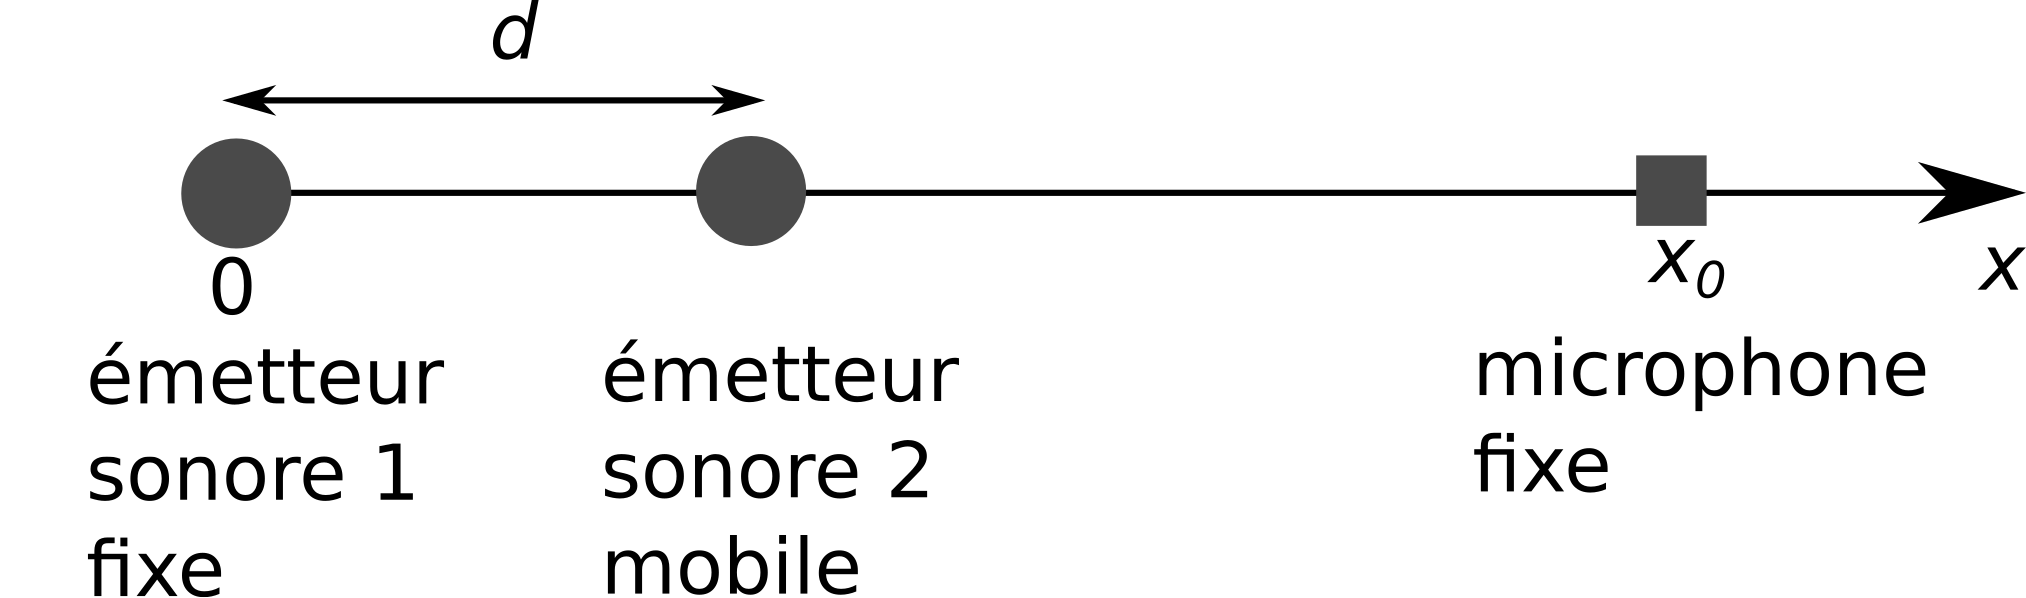
\includegraphics[width=\linewidth]{microphone}
        \end{center}
    \end{minipage}
    \begin{enumerate}[label=\sqenumi]
        \item Lorsque $d=0$, qu'enregistre-t-on au niveau du microphone~?
        \item On part de $d=0$ et on augmente $d$ jusqu'à ce que le signal
            enregistré soit nul. Ceci se produit pour $d = \SI{6.0}{cm}$.
            Expliquer cette extinction.
        \item En déduire la longueur d'onde du son émis.
        \item Pour $d = \SI{12.0}{cm}$, quelle sera l'amplitude du signal
            enregistré~?
    \end{enumerate}
\end{NCexem}
\begin{enumerate}[resume]
    \item Déterminer l'expression du signal somme de deux ondes sinusoïdales de
        même fréquence \textbf{et même amplitude} en introduisant $\Delta
        \f(\Mr)$ et $\f_0(\Mr)$. Définir et déterminer son intensité lumineuse.
        On la mettra sous la forme de la formule de \textsc{Fresnel}. Exprimer
        les valeurs de $\D\f(\Mr)$ correspondant à des interférences
        constructives ou destructives. On pourra redonner\[\cos p + \cos q =
        2\cos \left( \frac{p+q}{2} \right)\cos \left( \frac{p-q}{2} \right)\]
    \item Démontrer le lien entre déphasage et différence de marche. Démontrer
        le lien entre déphasage et chemin optique. Donner les déphasages pour
        lesquels on a des interférences constructives et destructives.
        Déterminer les différences de chemin optique correspondant.
    \item Trous d'\textsc{Young}~: présenter l'expérience et montrer que la
        différence de chemin $\delta_{2/1}(\Mr)$ s'écrit \hfill $\delta =
        2ax/D$ avec $2a$ la distance entre les fentes. Donner les conditions sur
        $x$ pour avoir interférences constructives ou destructives. \smallbreak
        On pourra redonner
        \[\sqrt{1+\ep} = 1 + \ep/2 + o(\ep)\]
\end{enumerate}

\end{document}
